\documentclass{article}

\usepackage[english]{babel}
\usepackage{graphicx}

% Set page size and margins
% Replace `letterpaper' with `a4paper' for UK/EU standard size
\usepackage[letterpaper,top=2cm,bottom=2cm,left=3cm,right=3cm,marginparwidth=1.75cm]{geometry}

\usepackage[colorlinks=true, allcolors=blue]{hyperref}

\title{Developing For Game-boy}
\author{John Groton}

\begin{document}

\maketitle



\section{What?}

This project was my attempt at making a vertical shooter type game for the Game Boy using the original Z80 architecture of the Game Boy. My initial goals for this project was player movement with a player sprite, enemies or obstacles that can harm the player, and some way the player can interact with those obstacles/enemies. My stretch goals for this project included a score system that tracked high score and power-ups. Basically I wanted to make a game like \href{https://en.wikipedia.org/wiki/Space_Invaders}{Space Invaders} for the Game Boy. 

\section{Why?}

I'm minoring in game programming and I enjoy programming games a lot. I find seeing all the code becoming a functional game to be very rewarding. I took Game Architecture last semester and I found making a game with just a graphics library as a base very fun, so I take this as a new challenge.

I also love all things retro so when I found out I could make a game for the Game Boy I instantly got excited. I find that limitations foster creativity and I am really inspired by the tricks developers used back in the day to make awesome games. I think it would be a great exercise to do it myself.

\section{How?}

\subsection{Finding an Assembler}

The first thing I did was to find a development environment. Something that I actually had some trouble with. I found a couple I liked initially, but the one I liked did not have a windows version. I experimented with running it on a virtual machine, but I soon discovered they had an online version. I was very happy to learn about this and knew immediately that I would use that. 

This editor is the \href{https://rgbds.gbdev.io/}{RGBDS} editor, and it has a history dating back to 1996. RGBDS is a free and open source assembler and linker for making Game Boy games. It takes code and turns it instantly into a .gb file to be run in an emulator. I found it very convenient and user friendly during the project and would recommend it to anyone wanting to get into developing for the Game Boy.

\subsection{Getting Comfortable}

After finding the RGBDS assembler I wanted to get more comfortable with writing Z80 Assembly, and Z80 specifically for Game Boy. To do this I found and followed the \href{https://gbdev.io/gb-asm-tutorial/index.html}{GB ASM Tutorial} (GBAT). This tutorial is another open source project, and some of it is still in development. I followed the first two parts of this tutorial before starting work on my own game and found it to be very useful. Coding for the Game Boy can be a very frustrating and intimidating thing, so starting off with a tutorial was very nice. Additionally I used some of the code from this tutorial to help with more confusing aspects of development, for example writing to the tile map area of memory. I will talk more about what code I used from the tutorial as it comes up.

\subsection{Tiles and Tile Maps}

The first step to the game was simply getting something onto the screen. This sounds easy, but when developing for the Game Boy nothing is easy. The Game Boy uses a tile based graphics system. A great explanation for how Game Boy graphics work is this \href{https://www.youtube.com/watch?v=txkHN6izK2Y&t=120s}{video}. I used this video myself when doing research. A quick explanation is there are many different 8x8 pixel tiles somewhere in memory. These tiles need to be assembled in memory in the right order to show up on the screen. The tiles themselves are just strings of binary that the assembler interprets as pixels. The tile data includes things like position, and what color from the palette the pixel uses. 

\begin{figure}[htp]
    \centering
    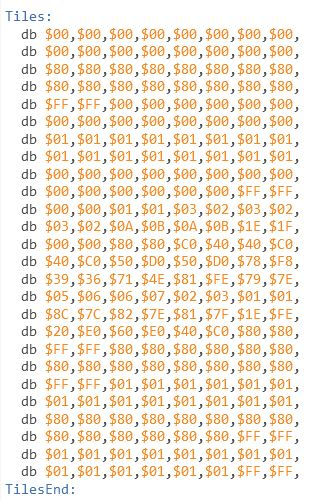
\includegraphics[width=8cm]{images/TilesCode.JPG}
    \caption{What tile data looks like in code}
    \label{Tiles Code}
\end{figure}

To make these tiles I first made markups in the pixel art software Aseprite. I then used another piece of software called \href{http://www.devrs.com/gb/hmgd/gbtd.html}{Game Boy Tile Designer} (GBTD) in order to turn the pixel art into code. GBTD is a piece of freeware that was made by Harry Mulder back in 1997, and was updated by various other programmers up until 1999. GBTD made the very confusing process of making tiles easy.

\begin{figure}[htp]
    \centering
    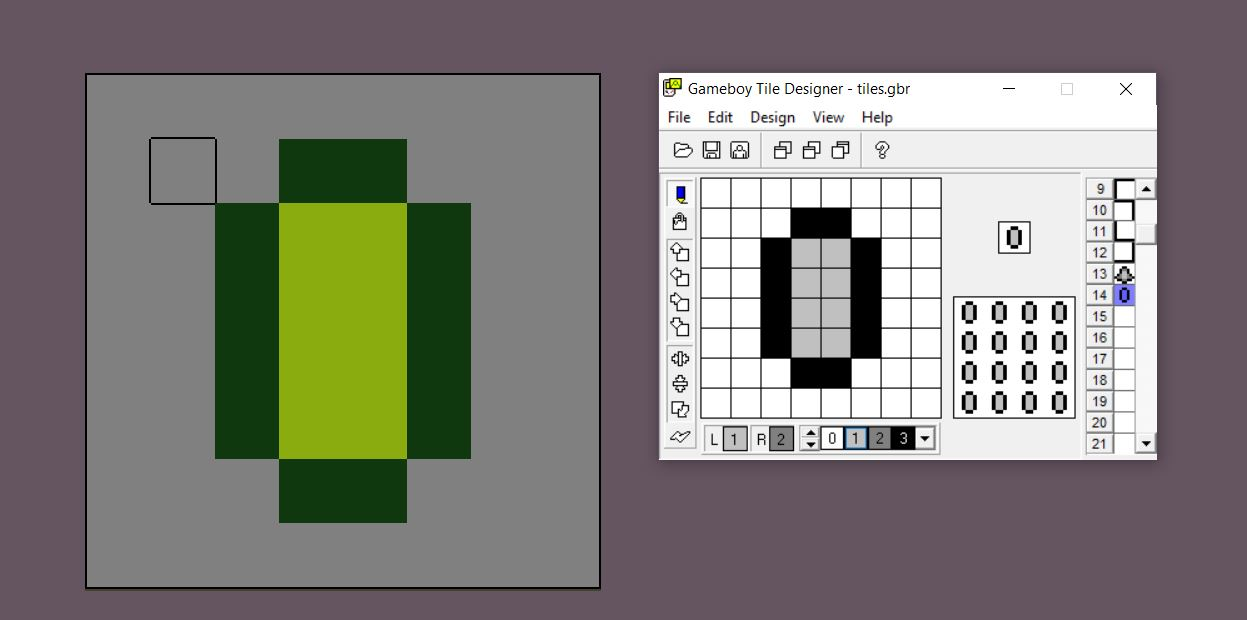
\includegraphics[width=8cm]{images/makingBullet.JPG}
    \caption{Aseprite on the left, and GBTD on the right}
    \label{Making the bullet sprite}
\end{figure}

The tiles then had to be loaded into memory, witch can be an involved process. There is a certain part of the Game Boy's memory that is reserved for tile data. To help with this I used a function from GBAT called \href{https://gbdev.io/gb-asm-tutorial/part2/functions.html}{MemCopy} This function copies tiles from one part of memory to another. I should also mention there are several types of tile data kept in different parts of memory. For example while tile map data is kept at memory location 9000, tile data for objects is kept at memory location 8000.

\begin{figure}[htp]
    \centering
    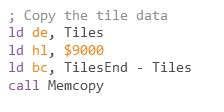
\includegraphics[width=6cm]{images/CopyTiles.JPG}
    \caption{Code that copies tile data in code, to the tile area of memory}
    \label{Calling memcopy}
\end{figure}

After the tile data is loaded into memory then the tile map can be assembled from those tiles. A tile map is just a list of each tile to place on the screen and what order to place those tiles in. I first tried to use software to build a tile map for me, but it's output did not work in RGBDS so I decided to make one by hand. This was easier then you would think, but it was very tedious.  

\begin{figure}[htp]
    \centering
    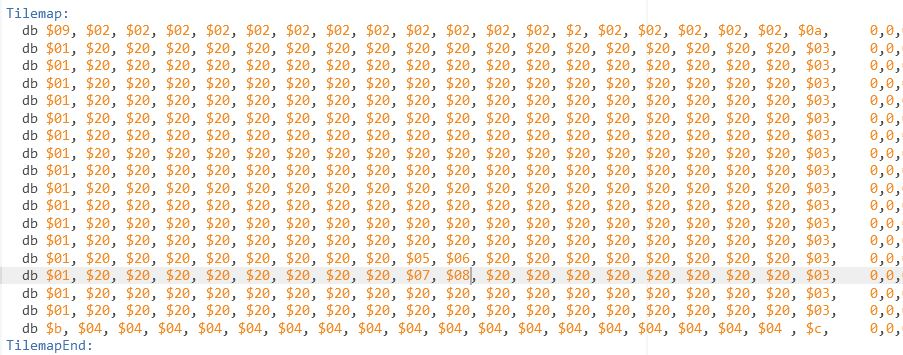
\includegraphics[width=6cm]{images/CorrectFirstTileMap.JPG}
    \caption{Tile Map Code}
    \label{Tile map code}
\end{figure}

\subsection{Objects}

Now that I had a tile map, I needed something to represent the player. Here is what I had on the screen at this moment.

\begin{figure}[htp]
    \centering
    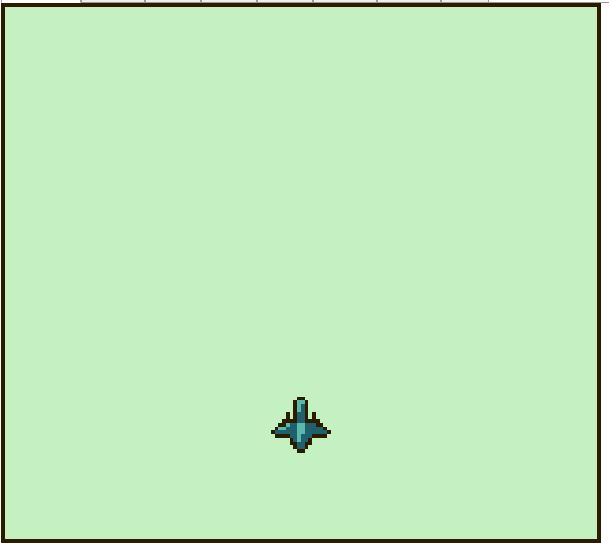
\includegraphics[width=6cm]{images/gettingShipOnScreen.JPG}
    \caption{First game screenshot}
    \label{What was on screen}
\end{figure}

What I had done, was load the player sprite (made up of four separate tiles) into the tile area of memory, then added it to the tile map. This was wrong, and I soon realized that I could not move a part of the tile map, without moving the whole tile map. What I really needed to do was to load the player sprite and location into Object Attribute Memory or OAM. OAM is a place in the Game Boy's memory that holds objects. Objects are used to represent most moving things like and enemy, a projectile, or a player. Each slot in OAM holds the objects position, one to two tiles that make up the object, and some other useful info. I was very sad to learn that objects can only be made up of one to two tiles, as now I had to redesign my player sprite. Making a sprite that was 16x16 pixels was hard enough. 

\begin{figure}[htp]
    \centering
    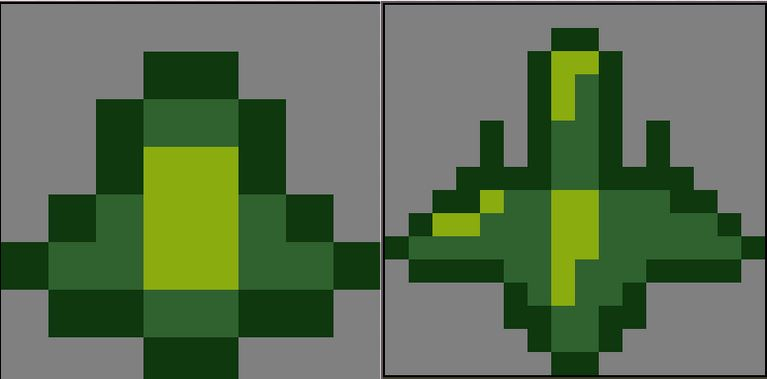
\includegraphics[width=6cm]{images/ShipComparasion.JPG}
    \caption{8x8 ship to the left, 16x16 ship on the right}
    \label{Ship comparasion}
\end{figure}

Now that I had made the right tiles, it was now time to write to OAM and make a new object for the player. To do this I used example code form \href{https://gbdev.io/gb-asm-tutorial/part2/objects.html}{GBAT}. Writing to OAM is a similar to writing to the tile area of memory. First though OAM must be cleared, when the Game Boy starts it fills the OAM with junk values. Those values must be gotten rid of before OAM is used. 

\begin{figure}[htp]
    \centering
    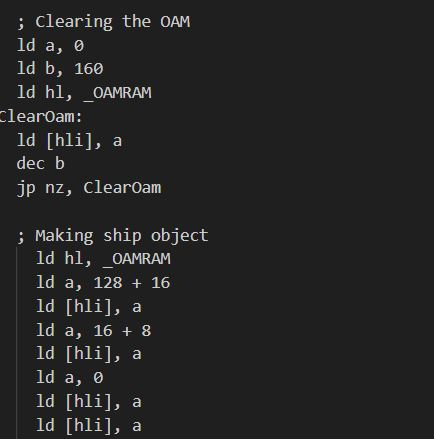
\includegraphics[width=6cm]{images/OAMExample.JPG}
    \caption{Code that clears OAM, then makes a new object}
    \label{OAM example code}
\end{figure}

This method of creating objects can be rather dangerous though as it is directly writing to memory. It can be very easy to mess up and break a lot of things. scalability can also be an issue with this method, as with each different object in OAM the off sett must be changed to access this new object. But for the simplicity of the game I wanted to make I chose to stick with this method.

\subsection{Manipulating Objects}

In order to move the player sprite, we need to change the x and y position in OAM. Luckily getting these values is pretty easy. For example if you wanted to get the y position of the second object in OAM you would access [OAMRAM + 4]. OAMRAM is the constant for the memory location of the start of OAM, and 4 is the off sett needed to get to the first element of the second object of OAM.

\begin{figure}[htp]
    \centering
    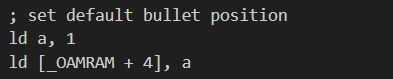
\includegraphics[width=6cm]{images/settingValueInOAM.JPG}
    \caption{Example of setting a value in OAM}
    \label{More OAM example code}
\end{figure}

Changing x and y positions of an objects in OAM is easy. The hard part is getting input from the player.

\subsection{Getting Input}

A great explanation of how input works in the Game Boy can be found \href{https://www.youtube.com/watch?v=ecTQVa42sJc}{here}, but I'll do my best to quickly explain it now. 

All of the input is stored in one byte at memory location FF00. Bits 7 and 6 mean nothing. Bit 5 however changes if the rest of the bits look at the direction pad, or at the rest of the buttons. So if bit 5 is 1, the rest of the bits represent the pad, and if bit 4 is 0 then the rest of the bits represent buttons a, b, select, and start. The code I used to get input was from GBAT, and you can find it \href{https://gbdev.io/gb-asm-tutorial/part2/input.html}{here}.

\begin{figure}[htp]
    \centering
    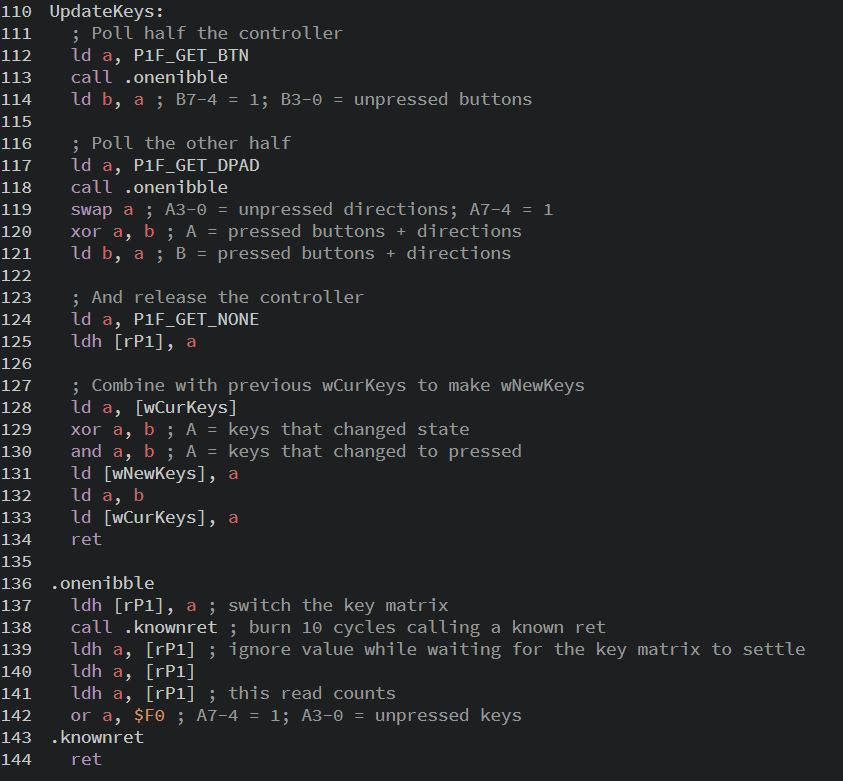
\includegraphics[width=10cm]{images/InputCode.JPG}
    \caption{Getting Input}
    \label{Get Input code}
\end{figure}

This code essentially takes the four bits from when the input byte is set to direction pad mode, and the combines it with the other four bits from when the input byte is set to button mode. This puts all the buttons in one neat byte for easy use.

\subsection{Interpreting Input}

Now that the input is all in one byte it can easily be interpreted. To do this constants are provided with all the bits set to 0 excepts the one corresponding to the button they are to represent. So to check if that button is pressed you AND your input, with the button constant, and if result bit is one that means the button was pressed. 

\begin{figure}[htp]
    \centering
    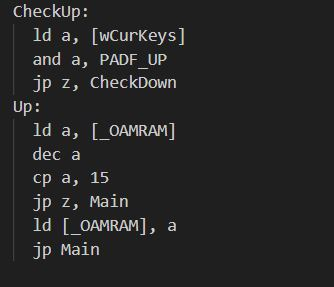
\includegraphics[width=4cm]{images/proccesingInput.JPG}
    \caption{Getting Input}
    \label{Procces Input}
\end{figure}

The code in Figure 10 checks the input data byte against the PADF-UP constant and will move the player if the input is the up button. A very similar process can be used to interpret all types of input. 

\subsection{Adding More}

To flesh out the rest I wanted to add shooting and enemies but this turned out to be a pretty large challenge, that I will talk more about in the challenges section. To be brief, I could only figure out a way to have one bullet and one enemy, pretty bad I know. I did not have to learn much more to do this, other then some collision code. I had the knowledge to code the rest of the game already, it just took time.

\section{Challenges}

I faced a lot of challenges in this project, most of it being just general debugging. In this section I will focus on breaking down the larger challenges, and summing up the many other small challenges I faced.

\subsection{Debugging}

Debugging for this project was at times very frustrating. The first difficulty was that debugging took longer then a normal program. As instead of simply running the code, I had the build the game then open an emulator and run it.

Another reason debugging was a challenge was the lack off, or unreliability of Internet sources. Usually when googling a bug for a more high level language there will be thousands of Stack Overflow questions about that bug. But with Z80 for Game Boy there was no real information outside of a couple of ancient forums. Thankfully the tutorial I used cleared up most questions, but for some bugs I was on my own, and it was a very frustrating process. 

\subsection{OAM Management}

One of the major challenges I had with development, and one I ultimately did not have the time to solve was dealing with multiple objects in OAM. Basically because I was dealing with OAM specifically I had to keep on incrementing what slot in OAM I was using. Since I was doing this by hand it meant dealing with more than a hand full of objects would be impossible. 

A potential solution to this would be using some sort of data structure to help me manage OAM. In one part of the GBAT a \href{https://gbdev.io/gb-asm-tutorial/part3/object-pools.html}{object pool} is actually recommended. I could add more objects using my current method, but it would soon become almost impossible to manage and make debugging even more painful then it already is. 

\subsection{Time}

This challenge was defiantly the biggest, and was mostly my fault. If I had started earlier on this project I would have had more time to deal with other challenges. I'm a little disappointed with how far I got and wished I had more time to add more to the game, and I might even after the semester is over.

\section{The Game!}

I thought since I've been talking so much about this game I should probably show you what it looks like. So I linked to a video showing off the game in my google drive \href{https://drive.google.com/file/d/1OmkPDGYeArlN-L3-UX6Kt9uyR1fwKF4a/view?usp=sharing}{here}.  

As you can see its a very simple game with only one enemy, and one bullet. I knew that I would be writing a lot of code, for very little end product but I was still surprised at how long it took me to make something so simple. Additionally all the source code is in a GitHub project linked \href{https://github.com/JohnnyG1234/ComputerArchFinal}{here}.

\section{Reflections}

To say this project went by fast is an understatement, I feel as though I woke up one day and I just had one weekend to finish. Even with this feeling I still learned a lot. I was fascinated learning how the guts of the Game Boy works, and how games were made for it. Discovering the vibrant community around making games for the Game Boy was also very fun, and I'm happy to learn how much support there is for learning Game Boy development to this day. Without the community around it, I would never have gotten as far as I did. 

It was also very interesting to look at the history of Game Boy development, and to even use a tool that was made two decades ago. I have a lot of respect for game developers of the past. They had to work way harder, for way less of a result, and had to come up with creative ways to get around hardware limitations, and that is worth celebrating.

\begin{figure}[htp]
    \centering
    
\includegraphics[width=4cm]{images/gameBoy.png}
    \caption{So Long Partner!}
    \label{Game Boy!}
\end{figure}

\begin{figure}[htp]
    \centering
    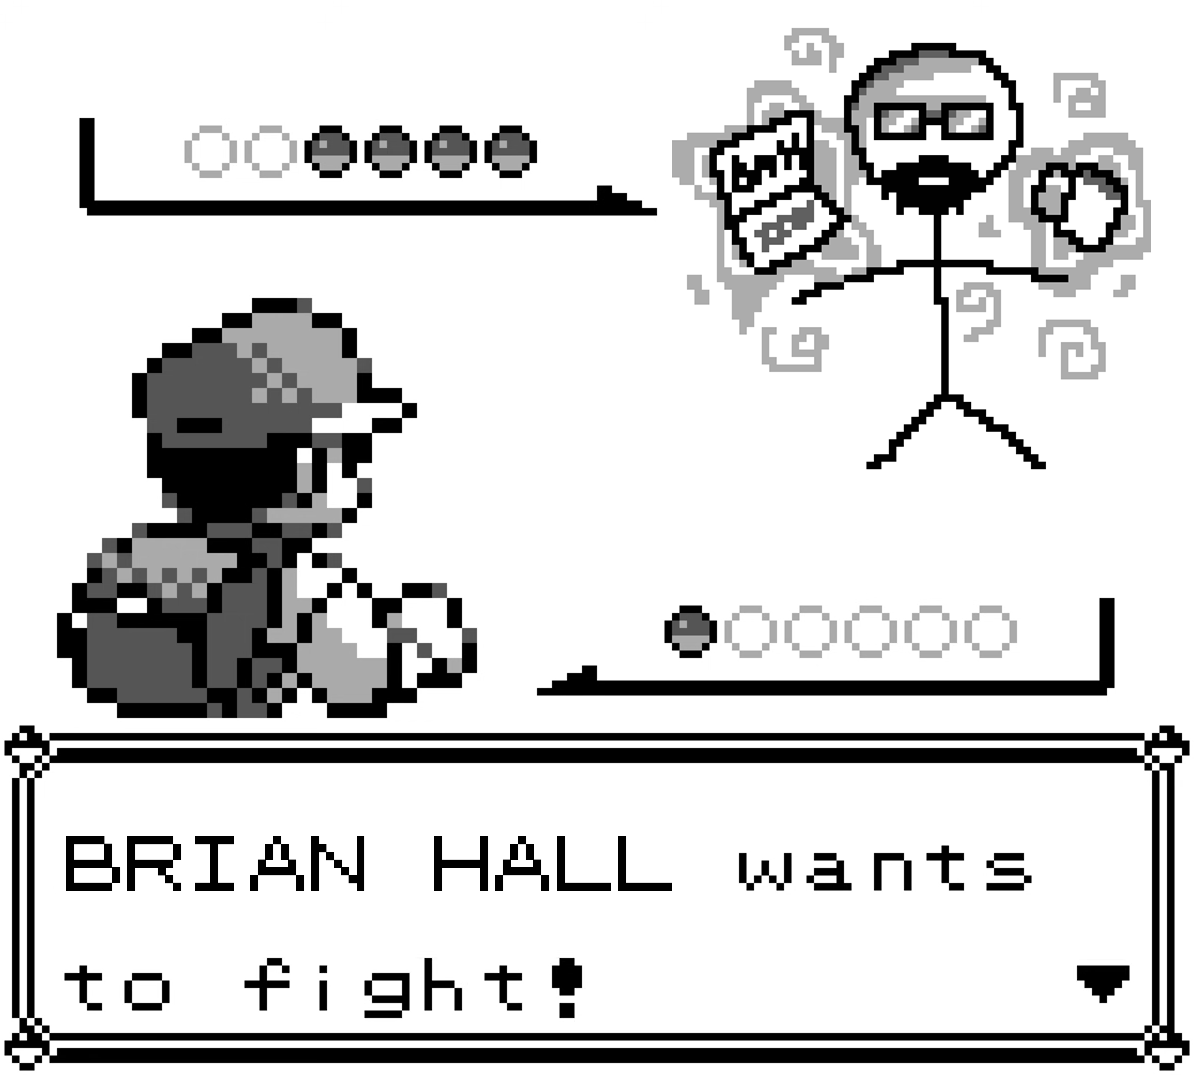
\includegraphics[width=12cm]{images/brianhallwantstofight.png}
    \caption{Nicole made this one!}
    \label{FIGHT}
\end{figure}


\section{Sources}

My biggest source was the \href{https://gbdev.io/gb-asm-tutorial/index.html}{GB ASM Tutorial}, I learned most of what I know from it, and took quite a bit of code from it to. 

Additionally I used many YouTube videos in researching. The first series I watched was a general overview of \href{https://www.youtube.com/watch?v=RZUDEaLa5Nw}{how the Game Boy works} made by the YouTuber \href{https://www.youtube.com/@jacktech5101}{Jack Tech}. 

Another series I watched covered how \href{https://www.youtube.com/watch?v=txkHN6izK2Y&t=122s}{Game Boy graphics work}, made by YouTuber \href{https://www.youtube.com/@systemoflevers/videos}{System of Levers}.

The last thing I want to cite is the software I used to make tiles called \href{http://www.devrs.com/gb/hmgd/gbtd.html}{Game Boy Tile Designer}, made by Harry Mulder.

Without these sources, and the amazing people who made them I would have probably never gotten a sprite to even appear on the screen.

\end{document}

